\chapter{Scalability Evaluation}
\label{cap:avaliacao}

This section presents the experiments to demonstrate the scalability of InterSCSimulator. To perform the tests we executed the simulator with different workloads, all based on the data presented in the S\~ao Paulo simulation. We started using 20\% of the simulated population and increased the load until the simulation of 100\% of the population. These experiments allow us to verify the increase in the usage of the computational resources by the number of simulated agents. Section \ref{sec:data_exp} presents the data used in all the executed tests, Section \ref{sec:tests_executions} presents all the simulator executions and the use of computing resources such as CPU, memory, and disk, and Section \ref{sec:conclusions_exp} presents our findings from the experiments.

\section{Experimental Data}
\label{sec:data_exp}

To perform the experiments, we created subsets of the OD survey of S\~ao Paulo. The first subset with 20\% of the total trips and four other increasing 20\% in each one until the complete OD. It is important to verify how is the evolution in the use of computational resources with the increasing workload. We executed the experiments in the Google Compute Engine (GCE), a cloud environment which provides virtual machines (VMs) with different capabilities. Table \ref{table:comparacao_experimentos} summarizes the data set of each experiment and the VM capability used to execute the experiment. We used the minimal necessary VM to each test due to the costs of using the VMs. 

\begin{table}[!htb]
\centering
{%
\begin{tabular}{|l|c|c|c|c|c|c|c|}
\hline

& \begin{sideways}Total Trips \end{sideways} 
& \begin{sideways}Car Trips \end{sideways} 
& \begin{sideways}Pedestrian Trips\hspace{0.5cm} \end{sideways} 
& \begin{sideways}Subway Trips \end{sideways} 
& \begin{sideways}Bus Trips \end{sideways} 
& \begin{sideways}VM Resources \hspace{1cm}\end{sideways} 
\\
\hline
Test 20
& 3.681.168 & 1.011.600 & 1.257.497 & 606.161 & 805.909 & 16CPU 32GB\\
Test 40
& 7.362.337 & 2.023.200 & 2.514.994 & 1.212.323 & 1.611.818 & 16CPU 50GB \\
Test 60
& 11.043.506 & 3.034.801 & 3.772.492 & 1.818.485 & 2.417.727 & 16CPU 70GB\\
Test 80
& 14.724.675 & 4.046.401 & 5.029.989 & 2.424.647 & 3.223.636  & 16CPU 90GB \\
Test 100
& 18.405.844 & 5.058.002 & 6.287.487 & 3.030.809 & 4.029.546  & 16CPU 104GB \\
\hline
\end{tabular}}
\caption{Comparison among the executions of InterSCSimulator\label{table:comparacao_experimentos}}
\end{table}%

Figure \ref{fig:travel_count_mode} presents the number of travels in the OD survey. There are a million travels by car, a million travels by buses,  million travels on foot, and million travels by subway or suburban train. The figure shows that most of the city population makes their trips walking or using public transportation, especially buses. However, there are also a huge number of cars in the city streets. The OD survey has data about other transportation modes such as cars passengers, bicycles, taxis, and school buses. We did not consider these modes because some of them do not impact the traffic such as car passengers or we do not have real data to make useful simulation such as bicycles, taxis, and school buses.

All the tests are available as Docker \citep{merkel2014docker} images to facilitate the tests execution and allow the reproducibility of the work.

\section{Tests Execution}
\label{sec:tests_executions}

Test20 simulated 20\% of the total travels of the OD. We ran this test 5 times and the mean execution time was 83 minutes with a standard deviation of 2 minutes. The tests used a mean of 68\% of the CPU with peaks of 90\% and a peak of 97\% of the memory (16GB). There was almost 800.000 maximum simultaneous actors during the simulation and its possible to see a significant increase in memory usage during the peak times of the city (8 am and 6 pm). Figure \ref{fig:exp20} presents a chart that summarizes the simulation execution information. 

\begin{figure}[!htb]
\centering
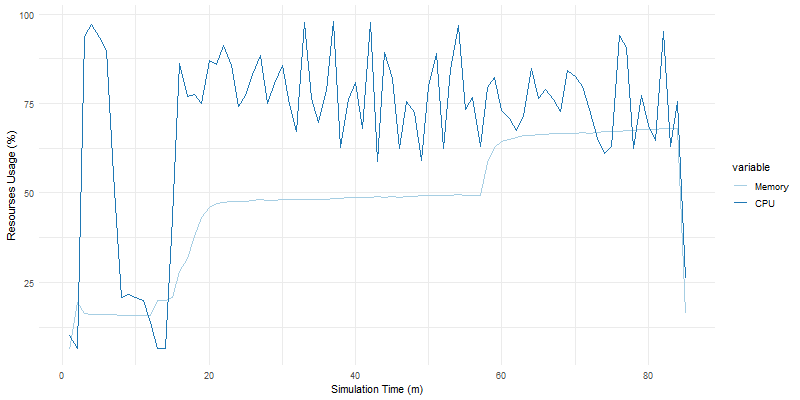
\includegraphics[width=1\textwidth]{figuras/chap-exp/experiment20.png}
\caption{Experiments with 20\% trips of the OD Survey}
\label{fig:exp20}
\end{figure}

Test40 simulated 40\% of the total travels of the OD. We performed this test 5 times and the mean execution time was 243 minutes with a standard deviation of 2 minutes. The tests used a mean of 65\% of the CPU with peaks of 82\% and a peak of 70\% of the memory (16GB). There was almost 1.2 million maximum simultaneous actors during the simulation and its possible to see a considerable increase in memory usage during the peak times of the city (8 am and 6 pm). Figure \ref{fig:exp20} presents a chart that summarizes the simulation execution information. 

\begin{figure}[!htb]
\centering
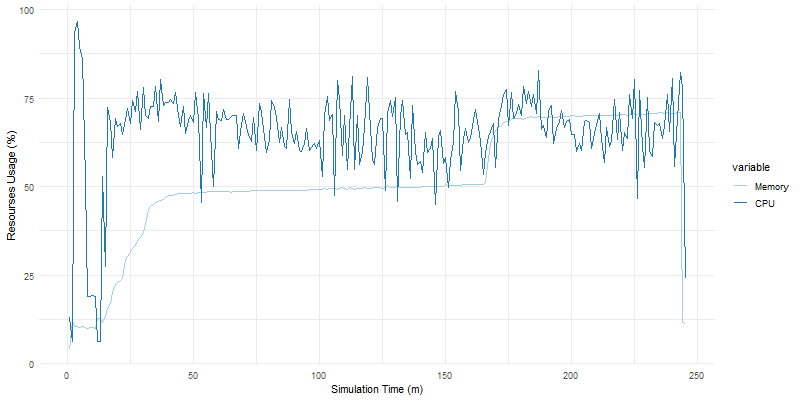
\includegraphics[width=1\textwidth]{figuras/chap-exp/experiment40.png}
\caption{Experiments with 40\% trips of the OD Survey}
\label{fig:exp20}
\end{figure}

\section{Results}
\label{sec:results_exp}

The charts in Figure \ref{fig:exp20} summarize the results of the scalability experiments.

QUANDO TIVER OS RESULTADOS FINAIS EXPLICAR O COMPORTAMENTO DE TODAS AS VARIÁVEIS (TEMPO DE EXECUÇÂO, CUSTO E RECURSOS USADOS)

\begin{figure}[!htb]
\centering
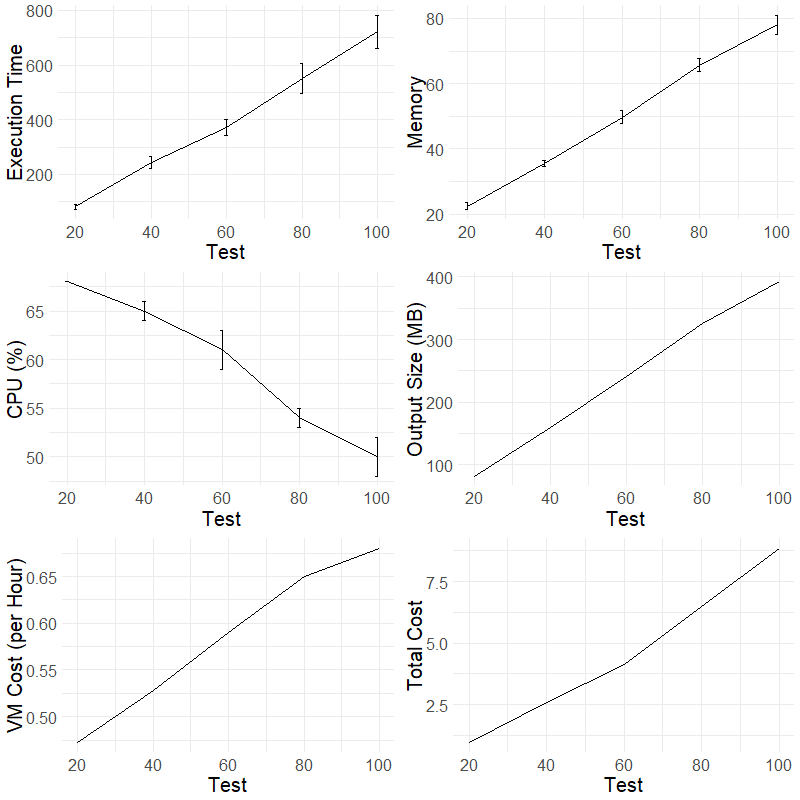
\includegraphics[width=1\textwidth]{figuras/chap-exp/dados.png}
\caption{Comparison among the five Experiments}
\label{fig:exp20}
\end{figure}


\section{Conclusions}
\label{sec:conclusions_exp}